% Source of the figure one-detour.pdf: the two detours of the lemma on one detour. Highs are on the upper row and lows on
% the lower row of the walk P. (a) The elements a, a' meet x below; the red walk goes a, z, x, z', a' and replaces the
% gray part of P. (b) The dual: b, b' meet y above; the red walk goes b, w, y, w', b'. Larger elements are drawn higher.
% Compile with pdfLaTeX; the PDF is included in the manuscript at its natural size.
\documentclass[tikz,border=1pt]{standalone}
\usepackage[T1]{fontenc}
\pdfinfoomitdate=1 \pdftrailerid{} \pdfsuppressptexinfo=-1
\definecolor{pathred}{RGB}{200,40,40}
\tikzset{
  vertex/.style={circle, fill=black, inner sep=0pt, minimum size=2.2mm},
  newvertex/.style={circle, fill=pathred, inner sep=0pt, minimum size=2.2mm},
  pathedge/.style={line width=1.8pt, pathred, line cap=round},
  oldedge/.style={line width=0.7pt, gray!80, dash pattern=on 3pt off 2pt}}
\newcommand{\zig}[3]{% from column #1 to column #2, style #3: odd columns are at height 1, even columns at height 0
  \foreach \c [evaluate=\c as \n using int(\c+1)] in {#1,...,\numexpr#2-1\relax} {
    \pgfmathsetmacro{\ya}{Mod(\c,2)}
    \pgfmathsetmacro{\yb}{Mod(\c+1,2)}
    \draw[#3] (\c,\ya) -- (\n,\yb);
  }}
\begin{document}
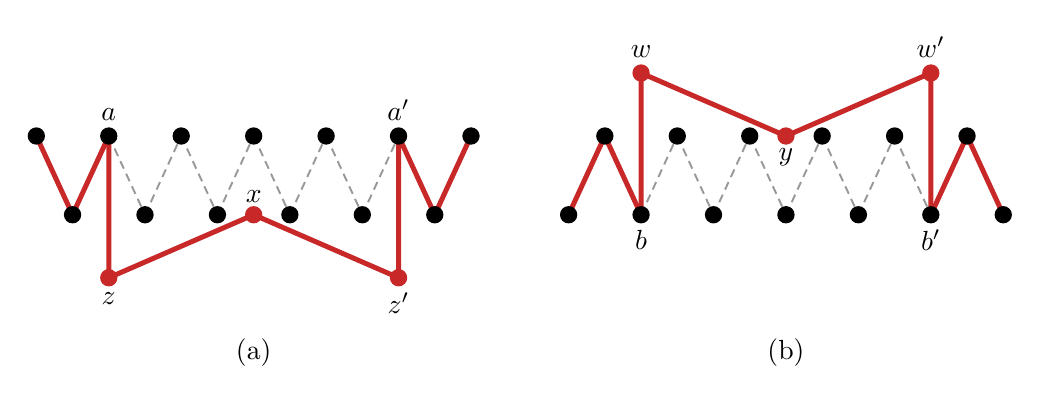
\begin{tikzpicture}[x=0.46cm, y=1cm]
  % panel (a): a at column 1, a' at column 9
  \begin{scope}
    \zig{1}{9}{oldedge}
    \zig{-1}{1}{pathedge}
    \zig{9}{11}{pathedge}
    \draw[pathedge] (1,1) -- (1,-0.8) -- (5,0) -- (9,-0.8) -- (9,1);
    \foreach \c in {-1,1,3,5,7,9,11} \node[vertex] at (\c,1) {};
    \foreach \c in {0,2,4,6,8,10} \node[vertex] at (\c,0) {};
    \foreach \p in {(1,-0.8),(5,0),(9,-0.8)} \node[newvertex] at \p {};
    \node[above=2pt] at (1,1) {$a$};
    \node[above=2pt] at (9,1) {$a'$};
    \node[below=2pt] at (1,-0.8) {$z$};
    \node[below=2pt] at (9,-0.8) {$z'$};
    \node[above=1pt] at (5,0) {$x$};
    \node at (5,-1.75) {(a)};
  \end{scope}
  % panel (b): b at column 2, b' at column 10, one row of the walk shifted by one column
  \begin{scope}[xshift=6.3cm]
    \zig{2}{10}{oldedge}
    \zig{0}{2}{pathedge}
    \zig{10}{12}{pathedge}
    \draw[pathedge] (2,0) -- (2,1.8) -- (6,1) -- (10,1.8) -- (10,0);
    \foreach \c in {1,3,5,7,9,11} \node[vertex] at (\c,1) {};
    \foreach \c in {0,2,4,6,8,10,12} \node[vertex] at (\c,0) {};
    \foreach \p in {(2,1.8),(6,1),(10,1.8)} \node[newvertex] at \p {};
    \node[below=2pt] at (2,0) {$b$};
    \node[below=2pt] at (10,0) {$b'$};
    \node[above=2pt] at (2,1.8) {$w$};
    \node[above=2pt] at (10,1.8) {$w'$};
    \node[below=1pt] at (6,1) {$y$};
    \node at (6,-1.75) {(b)};
  \end{scope}
\end{tikzpicture}
\end{document}
